\PassOptionsToPackage{unicode=true}{hyperref} % options for packages loaded elsewhere
\PassOptionsToPackage{hyphens}{url}
%
\documentclass[]{book}
\usepackage{lmodern}
\usepackage{amssymb,amsmath}
\usepackage{ifxetex,ifluatex}
\usepackage{fixltx2e} % provides \textsubscript
\ifnum 0\ifxetex 1\fi\ifluatex 1\fi=0 % if pdftex
  \usepackage[T1]{fontenc}
  \usepackage[utf8]{inputenc}
  \usepackage{textcomp} % provides euro and other symbols
\else % if luatex or xelatex
  \usepackage{unicode-math}
  \defaultfontfeatures{Ligatures=TeX,Scale=MatchLowercase}
\fi
% use upquote if available, for straight quotes in verbatim environments
\IfFileExists{upquote.sty}{\usepackage{upquote}}{}
% use microtype if available
\IfFileExists{microtype.sty}{%
\usepackage[]{microtype}
\UseMicrotypeSet[protrusion]{basicmath} % disable protrusion for tt fonts
}{}
\IfFileExists{parskip.sty}{%
\usepackage{parskip}
}{% else
\setlength{\parindent}{0pt}
\setlength{\parskip}{6pt plus 2pt minus 1pt}
}
\usepackage{hyperref}
\hypersetup{
            pdftitle={A Jornada para a Ciência de Dados},
            pdfauthor={Tiago Alves},
            pdfborder={0 0 0},
            breaklinks=true}
\urlstyle{same}  % don't use monospace font for urls
\usepackage{longtable,booktabs}
% Fix footnotes in tables (requires footnote package)
\IfFileExists{footnote.sty}{\usepackage{footnote}\makesavenoteenv{longtable}}{}
\usepackage{graphicx,grffile}
\makeatletter
\def\maxwidth{\ifdim\Gin@nat@width>\linewidth\linewidth\else\Gin@nat@width\fi}
\def\maxheight{\ifdim\Gin@nat@height>\textheight\textheight\else\Gin@nat@height\fi}
\makeatother
% Scale images if necessary, so that they will not overflow the page
% margins by default, and it is still possible to overwrite the defaults
% using explicit options in \includegraphics[width, height, ...]{}
\setkeys{Gin}{width=\maxwidth,height=\maxheight,keepaspectratio}
\setlength{\emergencystretch}{3em}  % prevent overfull lines
\providecommand{\tightlist}{%
  \setlength{\itemsep}{0pt}\setlength{\parskip}{0pt}}
\setcounter{secnumdepth}{5}
% Redefines (sub)paragraphs to behave more like sections
\ifx\paragraph\undefined\else
\let\oldparagraph\paragraph
\renewcommand{\paragraph}[1]{\oldparagraph{#1}\mbox{}}
\fi
\ifx\subparagraph\undefined\else
\let\oldsubparagraph\subparagraph
\renewcommand{\subparagraph}[1]{\oldsubparagraph{#1}\mbox{}}
\fi

% set default figure placement to htbp
\makeatletter
\def\fps@figure{htbp}
\makeatother

\usepackage{booktabs}
\usepackage{amsthm}
\makeatletter
\def\thm@space@setup{%
  \thm@preskip=8pt plus 2pt minus 4pt
  \thm@postskip=\thm@preskip
}
\makeatother
\usepackage[]{natbib}
\bibliographystyle{apalike}

\title{A Jornada para a Ciência de Dados}
\author{Tiago Alves}
\date{2020-04-30}

\begin{document}
\maketitle

{
\setcounter{tocdepth}{1}
\tableofcontents
}
\hypertarget{uma-jornada-inesperada}{%
\chapter{Uma Jornada Inesperada}\label{uma-jornada-inesperada}}

\emph{Um curso básico e completamente grauito para geeks (e outras pessoas)}

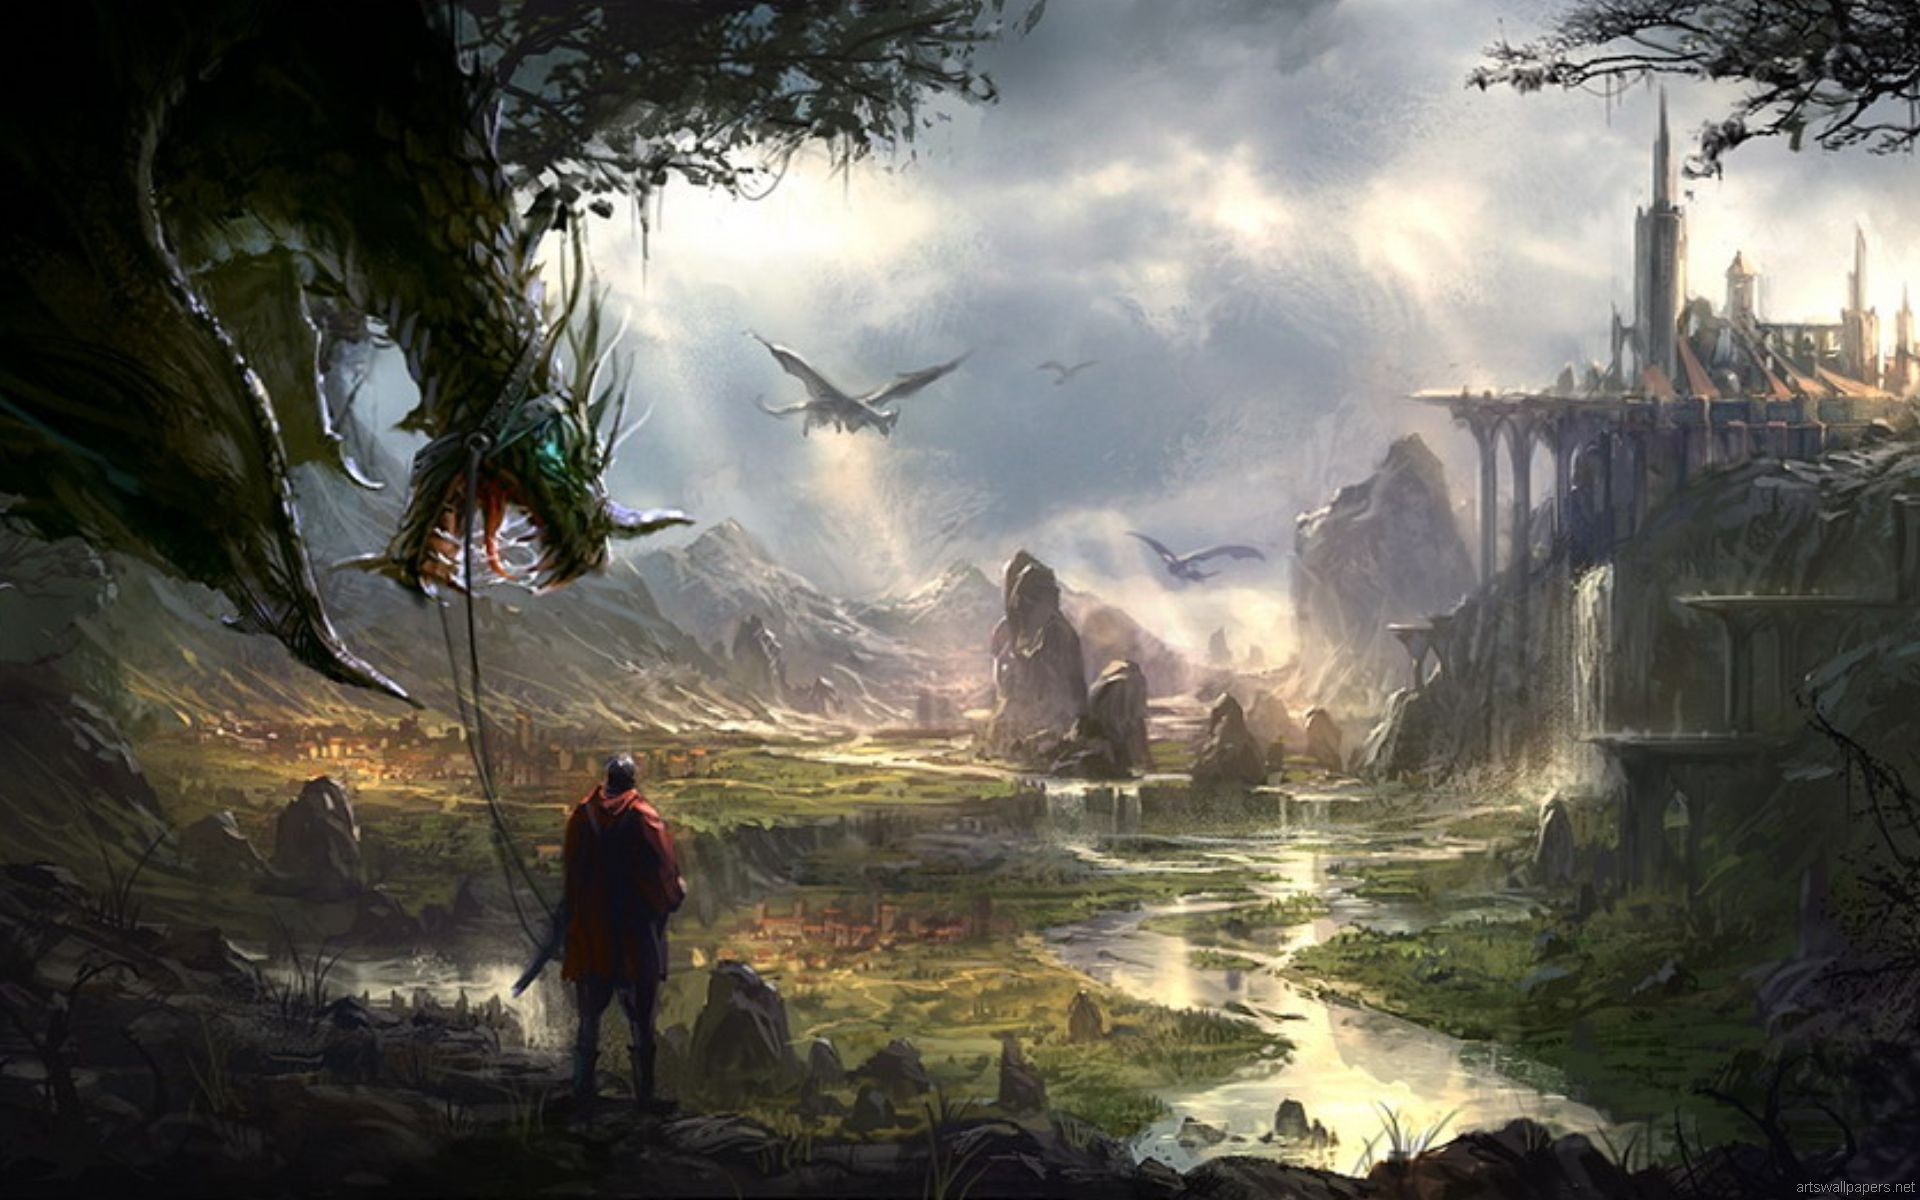
\includegraphics{images/index.jpg}

Bem vindo! Este é um curso básico de ciências de dados para pessoas que estão começando.
Aqui você encontrará muita matemática, dados e referências a cultura pop.

\hypertarget{sobre-mim}{%
\section{Sobre mim}\label{sobre-mim}}

\hypertarget{um-buxe1sico-sobre-python}{%
\chapter{Um básico sobre python}\label{um-buxe1sico-sobre-python}}

\hypertarget{configurando-o-ambiente}{%
\section{Configurando o ambiente}\label{configurando-o-ambiente}}

\hypertarget{o-primeiro-programa}{%
\section{O primeiro programa}\label{o-primeiro-programa}}

\hypertarget{bibliotecas-e-outras-ferramentas-uxfateis}{%
\section{Bibliotecas e outras ferramentas úteis}\label{bibliotecas-e-outras-ferramentas-uxfateis}}

\hypertarget{completando-o-pokedex---um-tutorial-sobre-como-obter-dados}{%
\chapter{Completando o Pokedex - Um tutorial sobre como obter dados}\label{completando-o-pokedex---um-tutorial-sobre-como-obter-dados}}

\hypertarget{como-saber-tudo-o-que-huxe1-sobre-os-pokuxe9mon---a-anuxe1lise-exploratuxf3ria}{%
\chapter{Como saber tudo o que há sobre os Pokémon - A análise exploratória}\label{como-saber-tudo-o-que-huxe1-sobre-os-pokuxe9mon---a-anuxe1lise-exploratuxf3ria}}

\hypertarget{descrevendo-os-pokuxe9mon---como-funciona-a-engenharia-de-features}{%
\chapter{Descrevendo os Pokémon - Como funciona a engenharia de features}\label{descrevendo-os-pokuxe9mon---como-funciona-a-engenharia-de-features}}

\hypertarget{lenduxe1rio-ou-nuxe3o---um-primeiro-modelo-de-classificauxe7uxe3o}{%
\chapter{Lendário ou não? - Um primeiro modelo de classificação}\label{lenduxe1rio-ou-nuxe3o---um-primeiro-modelo-de-classificauxe7uxe3o}}

\bibliography{book.bib,packages.bib}

\end{document}
